\documentclass[11pt]{article}

% Paquetes
%===================================================================================================

% Establecemos los márgenes
\usepackage[a4paper, margin=1in]{geometry}

% Separacion entre parrafos
\setlength{\parskip}{1em}

% Paquete para incluir codigo
\usepackage{listings}

% Paquete para incluir imagenes
\usepackage{graphicx}
\graphicspath{ {./images/} }

% Para fijar las imagenes en la posicion deseada
\usepackage{float}

% Para que el codigo acepte caracteres en utf8
\lstset{literate=
  {á}{{\'a}}1 {é}{{\'e}}1 {í}{{\'i}}1 {ó}{{\'o}}1 {ú}{{\'u}}1
  {Á}{{\'A}}1 {É}{{\'E}}1 {Í}{{\'I}}1 {Ó}{{\'O}}1 {Ú}{{\'U}}1
  {à}{{\`a}}1 {è}{{\`e}}1 {ì}{{\`i}}1 {ò}{{\`o}}1 {ù}{{\`u}}1
  {À}{{\`A}}1 {È}{{\'E}}1 {Ì}{{\`I}}1 {Ò}{{\`O}}1 {Ù}{{\`U}}1
  {ä}{{\"a}}1 {ë}{{\"e}}1 {ï}{{\"i}}1 {ö}{{\"o}}1 {ü}{{\"u}}1
  {Ä}{{\"A}}1 {Ë}{{\"E}}1 {Ï}{{\"I}}1 {Ö}{{\"O}}1 {Ü}{{\"U}}1
  {â}{{\^a}}1 {ê}{{\^e}}1 {î}{{\^i}}1 {ô}{{\^o}}1 {û}{{\^u}}1
  {Â}{{\^A}}1 {Ê}{{\^E}}1 {Î}{{\^I}}1 {Ô}{{\^O}}1 {Û}{{\^U}}1
  {ã}{{\~a}}1 {ẽ}{{\~e}}1 {ĩ}{{\~i}}1 {õ}{{\~o}}1 {ũ}{{\~u}}1
  {Ã}{{\~A}}1 {Ẽ}{{\~E}}1 {Ĩ}{{\~I}}1 {Õ}{{\~O}}1 {Ũ}{{\~U}}1
  {œ}{{\oe}}1 {Œ}{{\OE}}1 {æ}{{\ae}}1 {Æ}{{\AE}}1 {ß}{{\ss}}1
  {ű}{{\H{u}}}1 {Ű}{{\H{U}}}1 {ő}{{\H{o}}}1 {Ő}{{\H{O}}}1
  {ç}{{\c c}}1 {Ç}{{\c C}}1 {ø}{{\o}}1 {å}{{\r a}}1 {Å}{{\r A}}1
  {€}{{\euro}}1 {£}{{\pounds}}1 {«}{{\guillemotleft}}1
  {»}{{\guillemotright}}1 {ñ}{{\~n}}1 {Ñ}{{\~N}}1 {¿}{{?`}}1 {¡}{{!`}}1
}

% Para que no se salgan las lineas de codigo
% Para fijar una fuente que resalte
\lstset{breaklines=true, basicstyle=\ttfamily}

% Para que los metadatos que escribe latex esten en español
\usepackage[spanish]{babel}
\decimalpoint % Para que no se cambie el punto a la coma

% Para la bibliografia
% Sin esto, los enlaces de la bibliografia dan un error de compilacion
\usepackage{url}

% Para que se puedan clicar los enlaces
\usepackage{hyperref}

% Para mostrar graficas de dos imagenes, cada una con su caption, y con un caption comun
\usepackage{subcaption}

% Simbolo de los numeros reales
\usepackage{amssymb}

% Para que los codigos tengan una fuente distinta
\usepackage{courier}

\lstdefinestyle{CustomStyle}{
  language=Python,
  numbers=left,
  stepnumber=1,
  numbersep=10pt,
  tabsize=4,
  showspaces=false,
  showstringspaces=false
  basicstyle=\tiny\ttfamily,
}

% Para referenciar secciones usando el nombre de las secciones
\usepackage{nameref}

% Para enumerados dentro de enumerados
\usepackage{enumitem}

% Para mejores tablas
\usepackage{tabularx}

% Para poder tener el mismo identificador en dos tablas separadas
\usepackage{caption}

% Mostrar la página de las referencias en el indice del documento
\usepackage[nottoc,numbib]{tocbibind}

% Para mostrar las matrices
\usepackage{amsmath}

% Para que las notas al pie de pagina queden bien abajo
\usepackage[bottom]{footmisc}

% Para poner tablas en horizontal, ocupando bien la página
% cuando hay mucho texto en la table
\usepackage{lscape}

% Comandos personalizados
%===================================================================================================

% Para realizar las citas de forma corta
\newcommand{\customcite}[1]{\emph{"\ref{#1}. \nameref{#1}"}}

% Para entrecomillar un texto
\newcommand{\entrecomillado}[1]{\emph{``#1''}}

% Metadatos del documento
%===================================================================================================
\title{
    {Visión por Computador - Práctica Final} \\
    {Uso de redes siamesas para la clasificación de fotografías de ropa (Zalando)}
}

\author{
    {Sergio Quijano Rey}\\
    {sergioquijano@correo.ugr.es} \\
    {}\\
    {Alejandro Borrego Mejías} \\
    {alejbormeg@correo.ugr.es}\\
}

\date{\today}

% Separacion entre parrafos
\setlength{\parskip}{1em}

% Contenido del documento
%===================================================================================================
\begin{document}

% Portada del documento
\maketitle
\pagebreak

% Indice de contenidos
\tableofcontents

% Lista de figuras
% Uso el addtocontents para que no se muestre la seccion de indice de figuras en el indice inicial

\addtocontents{toc}{\setcounter{tocdepth}{-10}}
\listoffigures

\listoftables

% \lstlistoflistings
\addtocontents{toc}{\setcounter{tocdepth}{3}}

\pagebreak

\section{Abstract}

En este proyecto nos proponemos profundizar en el conocimiento de las Redes Siamesas y su funcionamiento para un problema de clasificación multiclase con KNN. Para el entrenamiento de la red emplearemos la función de error Triplet Loss y probaremos distintas técnicas de elección de triples, en concreto usaremos tripes aleatorios y triples \entrecomillado{difíciles} online. Por otra parte probaremos distintas arquitecturas para la red comenzando con una ResNet-18 de complejidad mucho mayor a la de la base datos y posteriormente usaremos una red mucho más sencilla que hemos denominado Light Model con la que mejoraremos sustancialmente los resultados obtenidos hasta el momento.

\section{Introducción}

\subsection{Problema a resolver}

En esta práctica vamos a trabajar con el uso de redes siamesas y la función de pérdida \emph{Triplet Loss}. Por tanto, calcularemos un \emph{embedding} de la base d y probaremos distintas técnicas de elección de triples como son los tripes aleatorios ptaremos dicha red para realizar una tarea de clasificación usando el algoritmo \emph{k-NN}.

Realizaremos dos experimentos. El primero de ellos basado en el entrenamiento de la red usando triples aleatorios. El segundo, basado en el entrenamiento de la red usando triples difíciles, calculados de forma \emph{online} por cada \emph{minibatch}.

\subsection{Elección del \emph{dataset}}

El dataset que hemos utilizado para la realización de este proyecto se denomina \emph{FashionMNIST} \cite{zalando_dataset:online} y nos proporciona un total de 60000 imágenes $28 \times 28$ en escala de grises de ropa de distintos tipos (en concreto de 10 clases distintas). 

Esta base de datos surge como una alternativa al famoso conjunto de datos \emph{MNIST}. Los autores de la base de datos buscaban mantener la estructura de la base de datos original (tamaño de las imágenes, número de clases, tamaños de los conjuntos de entrenamiento y test, \ldots) a la vez que proponer un mayor reto que el reconocimiento de dígitos \cite{database_why:online}.

Más adelante, en \customcite{adecuacion_arquitectura_red:seccion}, discutiremos sobre la ideonidad de la arquitectura de red teniendo en cuenta la base de datos que acabamos de presentar.

\subsection{Motivación} \label{motivacion:seccion}

Hemos elegido este proyecto por nuestro interés en el estudio de redes Siamesas. Queríamos profundizar en su funcionamiento, en concreto, en las dificultades que supone la generación de triples para el correcto entrenamiento de la red a través de la función de error \emph{Triplet Loss}. De hecho, y como comentaremos más adelante, esta ha sido la parte más complicada del proyecto, pues escribir un código lo más eficiente posible ha sido crítico para reducir drásticamente los tiempos de ejecución.

La elección de la base de datos viene motivada por la actualidad de los datos que en ella se presentan y por las características de la misma. En concreto, es una base de datos lo suficientemente sencilla como para permitirnos realizar la experimentación aquí presentada en tiempos razonables, a la vez que tratábamos un problema más o menos complejo de resolver.

\subsection{Objetivos a realizar}

Los objetivos que nos proponemos en este proyecto son: 

\begin{enumerate}
  \item Aplicar \emph{Transfer Learning}. Durante todos los experimentos, usaremos una red \emph{ResNet18} pre-entrenada sobre \emph{ImageNet} que modificaremos ligeramente (en la capa de salida) y sobre la que realizaremos \emph{fine tuning}.
  \item Entrenamiento de la red usando triples aleatorios. Esperamos obtener resultados muy malos. Sin embargo, tomamos esto como \emph{baseline}, con el que compararemos cuando propongamos una mejor forma de tomar los triples con los que entrenamos.
  \item Entrenamiendo de la red usando triples difíciles, calculados de forma \emph{online} dentro de cada \emph{minibatch}. Con esto esperamos obtener una mejora drástica frente al uso de triples aleatorios.
  \item Adaptación de ambas redes (la entrenada con triples aleatorios y la entrenada con triples difíciles) a una tarea de clasificación usando \emph{k-NN} sobre el \emph{embedding} que las redes siamesas calculan.
\end{enumerate}

\subsection{Otros detalles}

Al principio del \emph{Notebook} definimos una variable \lstinline{RUNNING_ENV} que indica en que tipo de entorno nos encontramos. Cuando \lstinline{RUNNING_ENV == "local"}, indicamos que estamos corriendo el \emph{Notebook} en local, y cuando \lstinline{RUNNING_ENV == "remote"} indicamos que estamos corriendo en \emph{Google Colab}. Así podemos controlar las pequeñas diferencias entre estos dos entornos de desarrollo. Principalmente son dos las diferencias:

\begin{itemize}
    \item Cuando corremos en \emph{Google Colab} tenemos que introducir un código de verificación
    \item Las rutas de la carpeta donde guardamos las imágenes son diferentes
\end{itemize}

Además, al estar usando \lstinline{Pytorch} como librería principal, hemos tenido que escribir mucho código para llevar a cabo tareas básicas (como el bucle del entrenamiento, funciones para mostrar el progreso del entrenamiento conforme se está realizando, funciones para evaluar un clasificador, \ldots) Por ello hemos decidido separar el código de la siguiente forma:

\begin{itemize}
  \item Una carpeta \lstinline{lib/} en la que tenemos ficheros \lstinline{.py} con el código básico del que ya hemos hablado
  \item Un \emph{notebook} \lstinline{Notebook.ipynb}, en el que realizamos todo el trabajo interesante. Por ejemplo, aquí definimos todos los hiperparámetros que usamos finalmente, las funciones de pérdida usadas, la forma de calcular los triples, la evaluación del modelo, \ldots
\end{itemize}

En último lugar, cabe destacar que estamos guardando los modelos entrenados en disco. Esto lo controlamos con el parámetro global \lstinline{USE_CACHED_MODEL}, en la sección de hiperparámetros. Cuando esta variable vale \lstinline{False}, se realiza el entrenamiento de los modelos y se guardan en memoria. Cuando la variable vale \lstinline{True}, no se realiza el entrenamiento y se cargan los modelos desde disco. Esto ha sido crítico para poder realizar experimentaciones rápidas sin tener que volver a entrenar una y otra vez los mismos modelos bajo las mismas condiciones. Además, cuando nos hemos encontrado con problemas con el consumo de memoria \emph{GPU}, entrenar, reiniciar y cargar el modelo desde disco ha sido una solución temporal (finalmente resolvimos estos problemas por otro camino, usando adecuadamente la instrucción \lstinline{torch.no_grad()})

\pagebreak

\section{Fundamentos Teóricos} 

\subsection {\emph{Redes Siamesas}}

Una red siamesa es una arquitectura en la que se tienen dos redes idénticas, con el objetivo que, dadas dos imágenes de entidades iguales, obtengan dos representaciones cercanas. Y al revés, dadas dos entidades distintas, se debe obtener dos representaciones distantes.

Al trabajar con dos redes idénticas, lo que realmente manejamos es una única red que calcula representaciones de imágenes pasadas como entrada. Usaremos dicha red para calcular representaciones de pares o triples (en nuestro caso concretro, trabajaremos sobre todo con triples) de imágenes dadas como entrada.

Aclaramos lo que entendemos por representaciones cercanas y distantes. En primer lugar, la red calculará, dada una imagen de entrada $28\times28$, un embedding de la imagen. Esto es, una representación vectorial es un espacio $\mathbb{R}^d$ con $d << 28*28$ (ie. $d = 2$, $d = 4$, \ldots). 

Con esto, dadas dos imágenes $x, y$, sus representaciones $ f_{\theta}(x),  f_{\theta}(y)$ serán cercanas cuando $$|| f_{\theta}(x) - f_{\theta}(y)||_2 \approx 0$$ Del mismo modo serán lejanas cuando $$|| f_{\theta}(x) - f_{\theta}(y)||_2 >> 0$$ 

\pagebreak
\subsection{\emph{Triplet Loss}}

Esta será la función de pérdida que vamos a usar para optimizar nuestra red siamesa. A continuación introducimos el por qué de su uso.

Durante el entrenamiento, la red verá como ejemplos triples. Esto es, triples de la forma \emph{anchor}, \emph{positive}, \emph{negative}. \emph{anchor} será una imagen arbitraria, mientras que \emph{positive} será una imagen de la misma clase que \emph{anchor} y \emph{negative} será una imagen de otra clase. Queremos que la distancia entre ancla y positivo sea pequeña, y entre ancla y negativo sea grande. Por tanto, lo que queremos es:

$$||f_{\theta}(anchor) - f_{\theta}(positive)||^2 \leq ||f_{\theta}(anchor) - f_{\theta}(negative)||^2 $$

luego 

$$||f_{\theta}(anchor) - f_{\theta}(positive)||^2 - ||f_{\theta}(anchor) - f_{\theta}(negative)||^2 \leq 0$$

Para evitar la trivialidad $f_{\theta}(img) = 0; \forall img$ añadimos un margen $\alpha > 0$ de la siguiente forma:

$$||f_{\theta}(anchor) - f_{\theta}(positive)||^2 - ||f_{\theta}(anchor) - f_{\theta}(negative)||^2 + \alpha \leq 0$$

Con esto, definimos una función de pérdida que solo se activará cuando la desigualdad no se mantenga, con lo que:

$$Loss(a, p, n) := max(||f_{\theta}(a) - f_{\theta}(p)||^2 - ||f_{\theta}(a) - f_{\theta}(n)||^2 + \alpha, 0)$$

\pagebreak
\subsection{Adecuación de la arquitectura de red a la base de datos escogida} \label{adecuacion_arquitectura_red:seccion}

Las redes siamesas se han usado sobre todo en tareas de reconocimiento de caras y en verificación de firmas a mano \cite{siamese_wikipedia:online}. Estos dos problemas presentan las siguientes características fundamentales:

\begin{itemize}
  \item La red tiene que distinguir si dos imágenes se corresponden a la misma entidad o no (dos fotografías de dos personas se corresponden a la misma, dos firmas se han realizado por la misma persona)
  \item La red va a ver ejemplos de entidades no vistas durante el entrenamiento. Por ejemplo, tiene que distinguir si dos fotos de personas son de la misma persona, sin haber visto fotografías de esa persona previamente. En modelos de clasificación clásicos la red puede enfrentarse a fotografías nunca vistas, pero de una clase de la que ha visto otras fotografías. Así, esta es una diferencia fundamental con otros modelos de \emph{machine learning} con los que hemos trabajado 
  \item Potencialmente, la red tiene pocos ejemplos de cada entidad de los que aprender. 
\end{itemize}

En nuestra base de datos no se presentan las características fundamentales que hemos expuesto. La red se va a enfrentar a imágenes de clases que ya hemos visto previamente (fotografías nuevas de botas, por ejemplo. Pero la red ha sido entrenada con otras fotografias de otros tipos de botas). Además, tenemos muchos ejemplos de cada una de las diez clases con las que trabajamos.

Entonces, ¿por qué trabajamos con esta base de datos? En un primer momento, exploramos bases de datos más adecuadas para este problema, que no tuviésen que ver con el reconocimiento de caras o de firmas manuales. Por ejemplo, con una base de datos de figuras \emph{Lego} \cite{lego_database:online}. Sin embargo, esta base de datos era demasiado compleja, tal y como nos indicó el profesor de teoría de la asignatura (nos indicó el problema de que muchas figuras salían en posturas demasiado diferentes, como por ejemplo, de cara a la cámara y de espaldas). Nos encontramos con problemas parecidos buscando bases de datos más adecuadas a las características fundamentales presentadas previamente.

Por tanto, escogemos usar esta base de datos porque, a pesar de no ser adecuado el uso de la arquitectura para este problema, podemos profundizar en todos los aspectos expuestos en \customcite{motivacion:seccion}. De hecho, y como se comentará más adelante, la base de datos ha supuesto una gran dificultad en lo que tiempos de entrenamiento se refiere. Con esto, dudamos mucho de haber sido capaces de realizar un estudio en una base de datos más adecuada teniendo en cuenta los recursos computacionales de los que disponemos (principalmente, los que \emph{Google Colab} nos otorga).

En \customcite{conclusiones_triples_aleatorios:seccion} vemos que con nuestra técnica \emph{baseline} se obtienen resultados muy pobres. Por lo tanto, la base de datos escogida no supone un problema trivial para la arquitectura de red que estamos empleando.

Una posible mejora que no exploramos por falta de tiempo es realizar el entrenamiento considerando 9 de las 10 clases, y evaluar el comportamiento sobre imágenes de la clase que nunca ha visto la red. Por ejemplo, nunca mostrar a la red imágenes de botas, y en evaluación, comprobar si la red es capaz de distinguir efectivamente imágenes de botas del resto de clases que sí ha visto durante el entrenamiento.

\pagebreak

\subsection{Métrica \emph{Silhouette}}

Usaremos esta métrica para medir la calidad de los clusters obtenidos con los modelos entrenados. Una buena clusterización es aquella en la que los elementos del mismo cluster están muy cerca entre sí (distancia intra-cluster pequeña) y los elementos de clusters distintos están lejos entre sí (distancia inter-cluster grande). Todo esto se resume en esta métrica.

Dado un punto $i$, definimos su índice de Silhouette $s(i)$ como:

$$s(i) := \frac{b(i) - a(i)}{max\{a(i), b(i)\}}$$

donde $a(i)$ es la distancia media del punto $i$ al resto de puntos del mismo cluster

$$a(i) := \frac{1}{|C_i|} \sum_{j \in C_i} d(i, j)$$

y $b(i)$ es la mínima distancia del punto $i$ a un punto de un cluster distinto:

$$b(i) := \min_{j \in C_k ; C_k \neq C_i} d(i, j)$$ 

Al ser $a(i), b(i)$ reales positivos, es claro que $s(i) \in [-1, 1]$. Como queremos que $a(i)$ sea pequeño y $b(i)$ sea grande, el mejor valor para $s(i)$ es $1$. 

Una vez que hemos definido el índice de Silhouette para un punto, definimos la métrica de Silhouette para toda una clusterización como la media de los índices de Silhouette punto a punto:

$$s = \frac{1}{n} \sum s(i)$$

Cuando $s \approx 0$ significa que las fronteras entre los distintos clusters no están muy diferenciadas.

% TODO -- hay que escribir esto

\pagebreak

\section{Entrenamiento usando triples aleatorios}

\subsection{Detalles de implementación}

Para la creación de los triples aleatorios, diseñaremos un \lstinline{Dataset} de \lstinline{Pytorch} para definir dichos triples aleatorios. Pasaremos de tener un conjunto de datos formado por pares (Imagen, Etiqueta) a tener un conjunto de datos formado por triples (Ancla, Positivo, Negativo). Notar que en dicha transformación las etiquetas pierden el protagonismo, lo que será clave a la hora de adaptar el bucle de entrenamiento, que ignorará dichas etiquetas por completo. 

En dicho \emph{dataset} definiremos un tamaño del conjunto de datos arbitrario. Podríamos considerar todos los triples del conjunto de datos. Pero esto supondría un \emph{dataset} de tamaño intratable. Además, dejaría de ser un conjunto con triples aleatorios y pasaría a ser un conjunto con todas las combinaciones de triples.  

Además de esto, el único detalle interesante es el pre-cómputo de las listas de índices en función de la clase. Es decir, tenemos acceso a los índices de las ímagenes de cada clase pre-computados, para que el cálculo de los triples sea más rápido.

Una vez hecho esto, el bucle de entrenamiento es el usual. Pasamos a la red \emph{minibatches} conteniendo los triples, la red calcula su representación, y aplicamos la función de pérdida a cada triple. Dicha función de pérdida está implementada en la clase \lstinline{TripletLoss} y \lstinline{TripletLossCustom} (la última se encarga de manejar el error de todo un \emph{minibatch}).

Utilizaremos para su entrenamiento minibatches de 32 triples y un total de 10 épocas. 

Fijamos el tamaño del embedding a 2, y el margen a 0.001. Para optimizar el modelo usamos \emph{Adam} con un \emph{learning rate} inicial de 0.001. Esto porque en \customcite{hyperparameter_tuning:seccion}, hemos hecho una exploración de parámetros para el modelo que usa triples difíciles online, llegando a que los parámetros óptimos (para ese modelo) son dichos valores. Lo ideal habría sido realizar una exploración de parámetros para los triples aleatorios. Sin embargo, por tratarse del modelo que vamos a usar de base con el que comparar, y por lo lento del proceso de exploración de parámetros (esto lo comentaremos en \customcite{hyperparameter_tuning:seccion}), nos conformamos con los parámetros encontrados para el otro modelo.

\pagebreak

\subsection{Resultados del entrenamiento} \label{resultados_entrenamiento:seccion}

La curva de aprendizaje se muestra en la siguiente gráfica:

\begin{figure}[H]
    \centering
    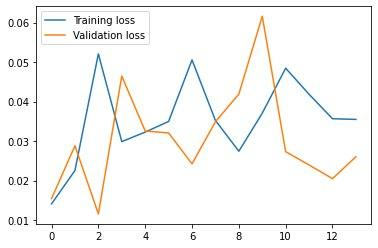
\includegraphics[width = 0.4 \textwidth]{random_curva_aprendizaje}
    \caption{Curva de aprendizaje para el entrenamiento del modelo usando triples aleatorios. En azul, la función de pérdida en entrenamiento. En naranja, la función de pérdida en validación}
\end{figure}

En dicha curva de aprendizaje se muetra un claro comportamiento errático en el aprendizaje. Esto puede deberse a los siguientes motivos:

\begin{itemize}
  \item El valor del \emph{learning rate} es demasiado alto y por eso el ajuste del error con \emph{back propagation} provoca dicho comportamiento errático
  \item No hemos entrenado durante suficientes épocas. Si entrenásemos durante más épocas, podríamos ver una tendencia global no tan errática
  \item El uso de triples aleatorios no es adecuado para optimizar la red, y por ello obtenemos dicho comportamiento errático
\end{itemize}

Comprobamos que no hemos usado pocas épocas entrenando durante 50, en vez de 10. La curva de aprendizaje en este caso es la siguiente:

\begin{figure}[H]
    \centering
    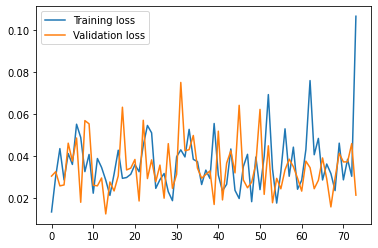
\includegraphics[width = 0.4 \textwidth]{random_curva_aprendizaje_larga}
    \caption{Curva de aprendizaje para el entrenamiento del modelo usando triples aleatorios. En este caso, en vez de entrenar durante 10 épocas, entrenamos durante 50}
\end{figure}

Seguimos observando el mismo comportamiento errático, y por tanto, descartamos que dicho comportamiento se explique por el uso de insuficientes épocas en el entrenamiento. Respecto al \emph{learning rate}, mostramos ahora el resultado de entrenar durante 10 épocas con un \emph{learning rate} mucho más bajo (en concreto, $0.0001$). La curva de aprendizaje en este caso es la siguiente:

\begin{figure}[H]
    \centering
    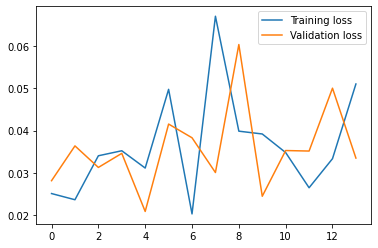
\includegraphics[width = 0.4 \textwidth]{random_curva_aprendizaje_lrbajo}
    \caption{Curva de aprendizaje para el entrenamiento del modelo usando triples aleatorios. En este caso, en vez de entrenar usando un \emph{learning rate} de 0.001, usamos 0.0001. De nuevo, estamos entrenando durante 10 épocas}
\end{figure}

El comportamiento errático sigue mostrándose con claridad. Por tanto, descartamos las dos primeras hipótesis para explicar el comportamiento errático, y consideramos la más probable la última: el uso de triples aleatorios no es adecuado para la optimización de la red.

Notar que en el \emph{Notebook} entregado usamos, tanto para el margen como para el \emph{learning rate} los parámetros originales. Si se quieren obtener los resultados que hemos mostrado para descartar hipótesis basta con modificar dichos parámetros en la celda con todos los hiperparámetros del \emph{Notebook}.

Obtenemos un valor de la función de pérdida, en el conjunto de test, de $0.0621$. Dicho valor se consigue usando la función \lstinline{test_model}, que se encuentra en nuestra librería, en el fichero \lstinline{core.py}. Más adelante, en \customcite{random_adaptacion_resultados_clasificacion:seccion}, mostraremos más métricas del modelo obtenido, una vez que lo hayamos adaptado a una tarea de clasificación.

\pagebreak

\subsection{Adaptación a una tarea de clasificación} 

Una vez entrenada la red, disponemos de una red que transforma imágenes en un espacio $\mathbb{R}^d$ con $d$ pequeña. Además, tenemos la propiedad fundamental que ya hemos comentado varias veces: imágenes de la misma clase tienen representaciones cercanas, e imágenes de clases distintas tienen representaciones lejanas.

Por ello, parece adecuado usar el algoritmo \emph{k-NN} para adaptar nuestra red, que simplemente calcula cierta representación de las imágenes, para una tarea de clasificación. Esto es lo que hacemos en la clase \lstinline{EmbeddingToClassifier}, que toma una red de este tipo y realiza la adaptación que ya hemos comentado.

Para ello, toma la red y el conjunto de imágenes que usaremos como base de instancias para \emph{k-NN}. Calculamos y almacenamos las representaciones de todas las imágenes. Cuando llega un nuevo ejemplo (una nueva imagen), calculamos su representación y aplicamos \emph{k-NN} sobre nuestro conjunto almacenado de representaciones. 

En nuestro caso, usaremos $k = 3$. Los resultados de realizar esta adaptación a la tarea de clasificación se muestran a continuación.

\pagebreak 

\subsubsection{Resultados de clasificación} \label{random_adaptacion_resultados_clasificacion:seccion}

Nos aprovechamos de los cálculos que realizamos en la adaptación del modelo a clasificación para mostrar la gráfica del \emph{embedding} obtenido sobre el conjunto de entrenamiento:

\begin{figure}[H]
    \centering
    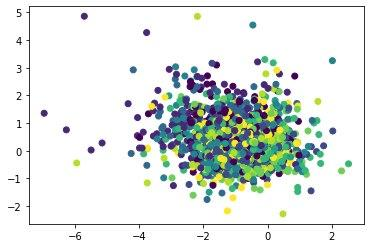
\includegraphics[width = 0.4 \textwidth]{random_embedding}
    \caption{Gráfica del \emph{embedding} calculado por la red sobre el conjunto de entrenamiento. Los colores muestran la clase asociada a cada uno de los puntos que mostramos}
\end{figure}

Como se puede ver en el gráfico anterior, las distintas clases se hallan muy juntas entre sí y entremezcladas, sin una separación clara por clase, por lo que la red no está separando correctamente las distintas clases del dataset. Este comportamiento era esperable debido a los malos resultados obtenidos previamente en el entrenamiento, y que mostrábamos en \customcite{resultados_entrenamiento:seccion}

Por otra parte, si ahora extraemos algunas métricas como son el Accurcy del clasificador, el Área bajo la curva ROC o la métrica Silohuette sobre el modelo de clasificación KNN obtenemos lo siguiente: 

\begin{table}[H]
\begin{center}
    \begin{tabular}{|c|c|c|c|}
        \hline
        Dataset & Accuracy & Área bajo la curva ROC & Silhouette \\
        \hline
        train & 0.125 & 0.5562 & -0.1894  \\
        test & 0.1042 & 0.5075 &  -0.1014 \\
        \hline
    \end{tabular}
\end{center}
   \caption{Métricas adicionales del modelo entrenado usando triples aleatorios}
\end{table}


Como podemos observar, el Accuracy obtenido tanto en entrenamiento como en test por el clasificador es muy bajo, de un 10\%. Por otro lado el Área bajo la curva ROC es de un 0.5, lo que nos indica que el comportamiento que tiene el clasificador es prácticamente aleatorio. Finalmente en la métrica Silohuette obtenemos un -0.1014 lo que nos indica que las fronteras de las distintas clases se encuentran entremezcladas, es decir, los elementos de las distintas clases no están bien separados unos de los otros. No obtenemos \emph{clusters} de calidad en el \emph{embedding} calculado.

En definitiva, estamos obteniendo unos resultados muy malos debido a una red que calcula un \emph{embedding} muy pobre. Como el algoritmo \emph{k-NN} depende fundamentalmente de la calidad de dicho \emph{embedding}, era de esperar, a la vista de los resultados de \customcite{resultados_entrenamiento:seccion}, un comportamiento muy malo en la adaptación a clasificación.

\pagebreak

\subsection{Conclusiones} \label{conclusiones_triples_aleatorios:seccion}

Los resultados obtenidos por el modelo de clasificación usando la Red Siamesa entrenada con triples aleatorios son muy pobres, como hemos mostrado tanto en \customcite{resultados_entrenamiento:seccion} como en \customcite{random_adaptacion_resultados_clasificacion:seccion}. Claramente no se pueden tomar como una solución al problema planteado en este proyecto. 

No obstante este modelo constituye un buen punto de partida sobre el cual mejorar los resultados obtenidos. En \customcite{resultados_entrenamiento:seccion} hemos defendido la hipótesis de que el comportamiento errático está causado por la inconveniencia de los triples aleatorios como mecanismo de selección de dichos triples. Por tanto, veremos más adelante si un mecanismo más adecuado de selección de triples consigue optimizar de forma correcta la red con la que estamos trabajando.

Cabe destacar de nuevo que no hemos realizado una exploración de los hiperparámetros que definen el modelo y su entrenamiento. Principalmente, el valor del margen para la función de pérdida, el \emph{learning rate} y la dimensión del \emph{embedding} resultante. No tenemos tiempo para realizar una exploración que requiere mucho tiempo de cómputo. Además, consideramos que este mal comportamiento no se va a corregir con una mejor selección de parámetros.

\pagebreak

\section{Entrenamiento usando triples \emph{online}}

\subsection{Detalles de implementación}

En este caso cambiaremos la estrategia para generar los triples (\emph{anchor}, \emph{positive}, \emph{negative}). En el uso de triples aleatorios, creábamos de forma \emph{offline} un conjunto de datos de triples, en el que ya no necesitábamos información de las etiquetas (pues va implícita en la estructura de triples). En este caso pasaremos a usar una estrategia \emph{online}.

Para ello, realizaremos un bucle clásico de entrenamiento:

\begin{enumerate}
  \item Tomamos un \emph{minibatch} de imágenes etiquetadas, 
  \item Pasamos las imágenes por la red obteniendo los valores de salida
  \item Con los valores de salida y las etiquetas, calculamos la función de pérdida
  \item Propagamos hacia atrás la pérdida
\end{enumerate}

Si en los triples aleatorios definíamos un \emph{dataset} para manejar los triples, en este caso usaremos una función de péridda de \lstinline{Pytorch} para dicho manejo de los triples. Esta función de pérdida la definimos en la clase \lstinline{OnlineTripletLoss}. 

La estrategia es la siguiente. Por cada imagen del \emph{batch}, calcularemos su triple más difícil dentro de dicho \emph{batch}. Es decir, consideramos una a una las imágenes del \emph{batch} como anclas. Dada un ancla, buscamos la imagen del \emph{batch} de la misma clase más alejada (positivo difícil), y la imagen de distinta clase más cercana (negativo difícil). Con este triple difícil calculamos el \emph{Triplet Loss}. Devolvemos la media de las pérdidas por cada triple.

Con esto conseguimos generar, de forma \emph{online}, triples difíciles, pero no extremadamente difíciles, pues el espacio de búsqueda de positivos y negativos se restringe al \emph{batch}. Para tener un buen compromiso en la dificultad, usaremos un tamaño de \emph{batch} considerablemente grande, en concreto, de 1024. Además, los \emph{minibatches} serán distintos entre épocas, y por tanto conseguimos ver combinaciones distintas entre épocas (esto no lo lograríamos usando minería de triples \emph{offline}).

Para acelerar el entrenamiento, por cada \emph{minibatch} que pasamos a la función de pérdida, realizamos pre-cómputos para que ciertas operaciones no se repitan por cada elemento del \emph{minibatch}. En concreto, y como ya hemos hecho previamente, calculamos una lista de listas, en el que cada lista almacena los índices de las imágenes de una clase en concreto. También calculamos una lista de listas, en el que cada lista almacena los índices de todas las imágenes que no son de una clase en concreto. Esta estrategia hace que los tiempos de entrenamiento se reduzcan aproximadamente 10 veces. 

Además, para que esta estrategia sea efectiva, es bueno usar \emph{minibatches} de gran tamaño, para que el tiempo que perdemos pre-computando se amortice con muchos cálculos ahorrados. Y ya usábamos \emph{minibatches} grandes para encontrar triples de suficiente dificultad.

\subsection{\emph{Hyperparameter tuning}} \label{hyperparameter_tuning:seccion}

Como este va a ser nuestro modelo final, vamos a considerar también hacer un \emph{Grid Search} de los parámetros más importantes del modelo, usando como técnica de validación \emph{4-Fold Cross Validation}. Los parámetros más relevantes a explorar consideramos que son: el learning rate, la dimensión del embedding y el margin (el parámetro $\alpha$ de la fórmula de \emph{TripletLoss}). 

Los valores que, inicialmente, consideramos explorar son:

\begin{itemize}
  \item Margen: $\{0.001, 0.01, 0.1\}$
  \item \emph{Learning Rate}: $\{0.0001, 0.001, 0.01\}$
  \item Dimensión del \emph{embedding}: $\{2, 3, 4\}$
\end{itemize}

Decimos que consideramos \entrecomillado{inicialmente} explorar porque ciertas combinaciones no las hemos explorado, al ver que ciertos valores de los parámetros producían resultados muy malos, y por tanto, consideramos que no merecía seguir explorando una zona potencialmente mala.

Para evaluar cada combinación de parámetros del Grid vamos a emplear \emph{4-fold Cross Validation}, dividiendo el conjunto de todas las imágenes de entrenamiento (un total de 48000) en 80 \% para Training y 20 \% para validación.

Lo ideal habría sido usar 5 o 10 \emph{fold cross validation}, al menos 10 épocas de entrenamiento. Sin embargo, haciendo cálculos, llegamos a la conclusión de que esto no era viable. Estimamos que tardábamos  un total de \emph{10 minutos por época}. 

En total queríamos explorar tres posibles valores de cada parámetro, lo que hace un total de \emph{27 combinaciones}. Por otro lado se consideró emplear 10 épocas y la estrategia 5-fold, el tiempo estimado de entrenamiento era el siguiente:   

$$\frac{10 \:  min * 10 \: epocas * 5 \: folds * 27 \: parametros}{60 \: min * 24 \: horas} = 9.375 dias$$

Como esta cantidad de tiempo de entrenamiento no se podía asumir, pensamos en reducir el número de épocas a 7, pues consideramos que este número seguía siendo apropiado para sacar conclusiones:

$$\frac{10 \:  min * 7 \: epocas * 5 \: folds * 27 \: parametros}{60 \: min * 24 \: horas} = 6.56 dias$$

Finalmente decidimos reducir el número de folds a 4 y hacer 4-fold Cross Validation, pero consideramos que ya no podíamos reducir ningún valor más sin perjudicar en exceso la búsqueda:

$$\frac{10 \:  min * 7 \: epocas * 4 \: folds * 27 \: parametros}{60 \: min * 24 \: horas} = 5.25 dias$$

Podemos ver que sigue siendo un tiempo intratable. Sin embargo, disponemos de dos cuentas de \emph{Google Colab} para explorar en paralelo, por lo que el tiempo se reduce a $2.625$ días, aproximadamente. Lo seguimos considerando un tiempo no razonable, pero durante el proceso de exploración supervisamos los resultados para podar ciertas zonas de exploración poco prometedoras de forma manual. Con ello, todo el conjunto de parámetros explorados y sus resultados se muestran en la siguiente tabla:

\begin{table}[H]
    \centering
    \begin{tabular}{|l|l|l|l|}
    \hline
        Embedding Dimension & Learning Rate & Margin & Loss \\ \hline
        2 & 0.0001 & 0.01 & 0.007372344437 \\ 
        2 & 0.0001 & 1 & 0.4078908339 \\ 
        3 & 0.0001 & 1 & 0.354682561 \\ 
        2 & 0.0001 & 0.1 & 0.04381236387 \\ 
        3 & 0.0001 & 0.1 & 0.05420429958 \\ 
        4 & 0.0001 & 1 & 0.3357170224 \\ 
        2 & 0.0001 & 0.001 & 0.01420788498 \\ 
        2 & 0.001 & 1 & 0.344632715 \\ 
        3 & 0.0001 & 0.001 & 0.0181999413 \\ 
        4 & 0.0001 & 0.001 & 0.01199295989 \\ 
        2 & 0.001 & 0.001 & 0.001895822257 \\ 
        3 & 0.001 & 0.001 & 0.001268613858 \\ 
        4 & 0.001 & 0.001 & 0.001237501063 \\ 
        \textbf{2} & \textbf{0.01} & \textbf{0.001} & \textbf{0.0007436529413} \\ 
        3 & 0.01 & 0.001 & 0.006536031724 \\ 
        4 & 0.01 & 0.001 & 0.001353246829 \\ 
        3 & 0.0001 & 0.01 & 0.02716585406 \\ 
      \hline
    \end{tabular}
    \caption{Resultados de la exploración de hiperparámetros usando \emph{4-fold Cross Validation}. En negrita, la combinación de parámetros que mejor resultados proporciona}
\end{table}

Como vemos en la anterior tabla, la mejor combinación de parámetros es la siguiente:

\begin{itemize}
  \item Margen: $0.001$
  \item \emph{Learning Rate}: $0.01$
  \item Dimensión del \emph{embedding}: $2$
\end{itemize}

\subsection{Resultados del entrenamiento}

\subsubsection{Resultados de clasificación}

\subsection{Conclusiones} \label{triples_online_resultados:seccion}

Como hemos podido observar en este experimento, los resultados han mejorado algo en comparación con el modelo entrenado con Triples aleatorios, (estamos triplicando prácticamente el \emph{accuracy} del modelo) pero siguen siendo muy pobres y claramente no se podría tomar como una solución al problema de clasificación multiclase planteado. 

Ante estos resultados nos vemos obligados de nuevo a cambiar la estrategia, como comentamos en \customcite{triples_light_motivacion:seccion}. 


\pagebreak

\section{Entrenamiento usando una red mucho más simple}

\subsection{Motivación} \label{triples_light_motivacion:seccion}

Los malos resultados que ya hemos comentado en \customcite{triples_online_resultados:seccion} nos fuerza a buscar posibles mejoras al modelo entrenado. Probamos en el último momento con una arquitectura de red mucho más simple. Esto lo hacemos siguiendo nuestra intuición, pues el conjunto de datos es relativamente sencillo (no deja de ser una alternativa al famoso conjunto de datos \emph{MNIST}). Y como comentaremos más adelante, conseguimos resultados mucho mejores con esta alternativa. 

Al haber explorado esta alternativa en el último momento, no tenemos tiempo para realizar todos los experimentos que habríamos considerado ideales. Entre ellos, haber realizado pruebas con la arquitectura de red (hemos usado la primera red que planteamos, no usamos técnicas de regularización sobre la red, por ejemplo), haber realizado exploración de los hiperparámetros con \emph{Cross Validation}, \ldots

\subsection{Detalles de implementación}

Para este nuevo enfoque al problema hemos creado una CNN mucho más simple que la que estábamos utilizando hasta el momento que hemos denominado \emph{LightModel}. La arquitectura de dicha red se muestra en la siguiente tabla:

\begin{table}[H]
\begin{center}
    
    \begin{tabular}{|c|c|c|c|}
        \hline
        Layer number & Layer Type & kernel size &  Input $|$ Output channels or neurons \\
        \hline
        1 & Conv2D & 3 & 1 $|$ 4 \\ 
        2 & Relu & - & - \\
        3 & Conv2D & 3 & 4 $|$ 8 \\ 
        4 & Relu & - & - \\
        5 & Conv2D & 3 & 8 $|$ 16 \\ 
        6 & Relu & - & - \\
        7 & Conv2D & 3 & 16 $|$ 32 \\ 
        8 & Relu & - & - \\
        9 & MaxPooling & 2 & - \\
        10 & Flatten & - & 32 $|$ 1 \\
        11 & Dense & - & 3200 $|$ 2 \\
    \hline
    \end{tabular}
\end{center}
    \caption{Descripción de la arquitectura del modelo \emph{LightModel}}
\end{table}

Como ya hemos comentado, esta es la primera arquitectura que diseñamos, y con la que conseguimos buenos resultados. Lo ideal habría sido probar con distintas modificaciones en la arquitectura para refinarla. Sin embargo, por falta de tiempo, nos conformamos con esta primera propuesta que da buenos resultados.

Por lo demás el resto de etapas de entrenamiento y posterior adaptación a un modelo de clasificación KNN serán iguales al las del los modelos anteriores, y por tanto, no volvemos a explicar este proceso. 

\subsection{\emph{Hyperparameter tuning}} 

De nuevo, y como ya hemos comentado, por falta de tiempo no realizamos \emph{Hyperparameter Tuning} con \emph{Cross Validation} para este nuevo modelo, que habría sido lo ideal. Por ello, decidimos nosotros los parámetros que vamos a emplear.

Con esta nueva arquitectura decidimos mantener el \emph{learning rate} del modelo anterior. En el \emph{hyperparameter tuning} anterior vimos que variar este parámetro no era muy significativo. Además, estuvimos explorando el efecto del margen en el error que se obtenía durante el proceso de etrenamiento. Llegamos a la conclusión de que este error era siempre menor cuanto más pequeño fuera el valor del margin y que no se producía overfitting. Por tanto, decidimos establecer como valor final para el margen $10^{-5}$. 

\subsection{Resultados del entrenamiento}

Comenzamos mostrando la curva de aprendizaje obtenida, en la siguiente figura:

\begin{figure}[H]
    \centering
    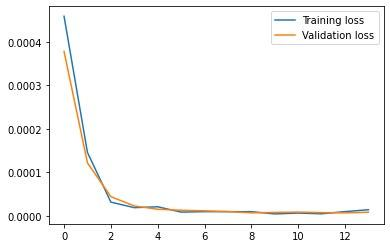
\includegraphics[width = 0.5 \textwidth]{triples_light_curva_aprendizje}
    \caption{Curva de aprendizaje para el entrenamiento del modelo usando triples difíciles \emph{online}. Además, usamos la nueva arquitectura de red. En azul, la función de pérdida en entrenamiento. En naranja, la función de pérdida en validación. En el eje $x$ mostramos las veces que se calculan las métricas, que corresponden con 10 \emph{batches}}
\end{figure}

Podemos ver que la red no comete sobreajuste, a pesar de que no hemos incluido elementos para tratar el sobre-aprendizaje en la arquitectura. Sin embargo, gracias a la simplicidad de la arquitectura, esto no supone un problema. 

Hemos entrenado la red durante tres épocas, lo hemos considerado así debido a la gran rapidez con la que desciende el error  al comienzo y porque tras la primera época la variación es mínima, por lo que entrenar durante más tiempo no iba a suponer una mejora considerable. En la curva de aprendizaje se ve claramente que a partir de los 40 primeros \emph{batches} no hay mejora alguna.

Por otra parte, tras el entrenamiento, se obtiene un error en el cojunto de Test de $8.61 \times 10^{-6}$, que nos confirma que no ha habido sobreajuste en el entrenamiento, como ya sospechábamos por los resultados mostrados en la curva de aprendizaje. 

\subsubsection{Resultados de clasificación}

Comenzamos mostrando, como hacíamos en secciones anteriores, la gráfica del \emph{embedding} obtenido:

\begin{figure}[H]
    \centering
    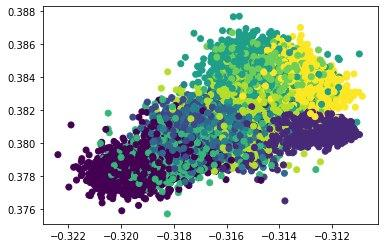
\includegraphics[width = 0.5 \textwidth]{triples_light_embedding}
    \caption{Gráfica del \emph{embedding} calculado por la red sobre el conjunto de entrenamiento. Los colores muestran la clase asociada a cada uno de los puntos que mostramos}
\end{figure}

Como se puede observar las clases se encuentran mejor separadas entre sí que en los modelos anteriores, aunque sigue habiendo cierto grado de solapamiento entre clases. Es más, hay ciertas clases que parecen mezclarse con otras, 

Mostramos ahora las matrices de confusión, pues puede ser que la red esté confundiendo clases que son parecidas (como con los distintos tipos de zapatos).

\begin{figure}[H]
    \centering

    \begin{subfigure}[b]{0.45 \textwidth}
        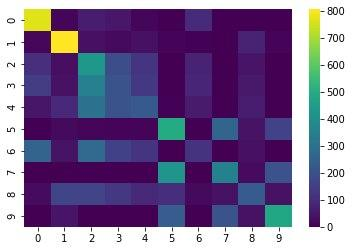
\includegraphics[width = 0.9 \textwidth]{triples_light_matrconf_entrenamiento}
        \caption{Conjunto de entrenamiento}
    \end{subfigure}
    \begin{subfigure}[b]{0.45 \textwidth}
        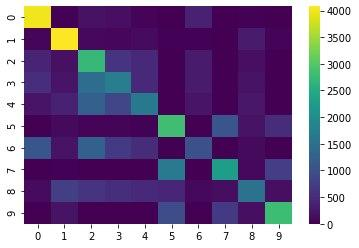
\includegraphics[width = 0.9 \textwidth]{triples_light_matrconf_test}
        \caption{Conjunto de test}
    \end{subfigure}

    \caption{Matrices de confusión obtenidas en la adaptación a la tarea de clasificación}
\end{figure}

Podemos observar que las dos primeras clases son bien distinguidas por la red entrenada. Sin embargo, en el resto de clases, no tenemos tanta precisión. Es destacable la confusión que tiene la red entre las clases 5, 7 y 9. Estas clases se corresponden con las sandalias, zapatillas tipo \emph{sneakers} y botas. Por tanto, la red tiene problemas para distinguir estos tres tipos de calzados.

Finalmente, mostramos las mismas métricas que hemos calculado en los modelos previos en la siguiente tabla: 

\begin{table}[H]
  \begin{center}
      \begin{tabular}{|c|c|c|c|}
          \hline
          Dataset & Accuracy & Área bajo la curva ROC & Silhouette \\
          \hline
          train & 0.51175 &  0.8476 & -0.0157\\
          test & 0.4101 & 0.7588 &  -0.0159 \\
          \hline
      \end{tabular}
  \end{center}
     \caption{Métricas adicionales del modelo ligero}
  \end{table}

Como se puede ver, el \emph{accuracy} mejora considerablemente con respecto a los modelos anteriores, logrando un 41 \% en el conjunto de \emph{test}. Además el \emph{área bajo la curva roc} también experimenta una mejora considerable, pues alcanza un $0.7588$ en \emph{test}, lo que nos indica que comienza a ser un mejor clasificador que los modelos anteriores. Como era de esperar, pues hemos visto que las clases están muy solapadas, el valor de \emph{Silhouette} es muy malo (cercano a cero)

\subsection{Conclusiones}

En primer lugar, el modelo planteado logra una mejora considerable respecto de los dos modelos previos. Sin embargo, los resultados siguen sin ser satisfactorios, y no podemos considerar el resultado obtenido como una solución al problema planteado.

En segundo lugar, consideramos que con esta alternativa se abre una nueva línea a investigar con la que se podría llegar a obtener un clasificador apropiado si se elige una arquitectura mejor de red ( manteniendo la simplicidad) o haciendo una búsqueda exhaustiva de los distintos hiperparámetros como se hizo con el modelo anterior. De tener el tiempo suficiente exploraríamos esta línea al parecernos la más prometedora.

Finalmente, podemos concluir que es fundamental adecuar la complejidad de la arquitectura de red a la complejidad del \emph{dataset} con el que se trabaja. Uno de los errores que hemos cometido en esta práctica ha sido trabajar con \emph{ResNet-18}, una arquitectura demasiado compleja para el problema a resolver. Por tanto, y a pesar de ser una red pre-entrenada, nos ha hecho perder mucho tiempo sin ofrecer resultados satisfactorios.

\pagebreak

\section{Conclusiones}

Finalmente, a modo de resumen de todas las conclusiones que se han obtenido hasta el momento: 

En primer lugar, nuestra hipótesis inicial sobre el uso de triples aleatorios queda confirmada. Es una técnica rápida para la generación de triples pero que no da buenos resultados, y por tanto es inútil más allá de servir como \emph{baseline} con el que comparar futuros modelos.

En segundo lugar, el uso de triples difíciles \emph{online} mejoró sustancialmente el modelo. Una buena selección de triples es clave para que la red mejore efectivamente. Además, la estrategia \emph{online} nos permite tanto seleccionar triples de forma relativamente rápida como equilibrar la dificultad de los triples escogidos. 

Sin embargo, vemos que aunque haya una mejora sustancial, no es suficiente. Al menos en la adaptación de la red a clasificación multiclase. Por tanto, buscamos mejorar los resultados de nuestro modelo, llegando a la conclusión de que es conveniente el uso de una red definida por nosotros, ligera y sin pre-entrenar.

Con esta red, mucho más simple, obtenemos unos resultados todavía mejores, en todas las métricas. Por tanto, aunque en general no sea una buena idea entrenar de cero un modelo, debido a la simplicidad de la base de datos es algo positivo: adecuamos la complejidad del modelo a las características de la base de datos y el entrenamiento desde cero no supone demasiado tiempo de cómputo. A pesar de esto, la red no obtiene unos resultados aceptables cuando realizamos la adaptación a clasificación. 

Un problema que hemos comentado previamente es todo el tiempo que hemos dedicado a la exploración de parámetros y optimización del modelo que usaba como base \emph{ResNet-18}. Si todo ese tiempo lo hubiésemos dedicado a mejorar la arquitectura de la red simple, a explorar sus parámetros y a mejorar el entrenamiento, estamos bastante convencidos que habríamos obtenido resultados mucho mejores.

Y para finalizar, en todos los casos hemos visto que, a pesar de obtener \emph{embeddings} aceptables, siempre ha habido una claro solapamiento entre las distintas clases. Una posible solución para este problema, que nos planteamos pero que no nos ha dado tiempo a implementar, es el uso de un margen adaptativo. Esto es, comenzar con un margen bajo y, con el paso de las épocas de entrenamiento, aumentarlo para forzar a que la red separe las distintas clases. De conseguir esto, pensamos que los resultados en la adaptación a clasificación habrían sido sustancialmente mejores.

\pagebreak

% Bibliografia
\bibliography{./References}
\bibliographystyle{ieeetr}

\end{document}
